\begin{frame}{Optimizing AI models for Edge}
\framesubtitle{Speech-To-Text Models}

\begin{block}{Quantization}

\begin{columns}[c,onlytextwidth]

\begin{column}{0.45\textwidth}
    \centering
    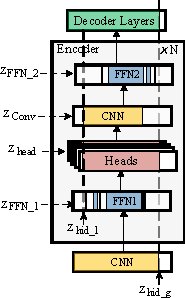
\includegraphics[width=0.4\linewidth]{figures/sparsity.pdf}
\end{column}

% ---------- TABLE ----------
\begin{column}{0.45\textwidth}
\centering

\small
\setlength{\tabcolsep}{4pt}
\renewcommand{\arraystretch}{1.2}

\makebox[\linewidth][c]{%
\fontsize{6}{7}\selectfont
\begin{tabular}{lcc}
\toprule
\textbf{Model Architecture} &
\multicolumn{2}{c}{\textbf{WER}} \\
\cmidrule(lr){2-3}
& \textbf{test-clean} & \textbf{test-other} \\
\midrule
Base (Conformer 118M Params) & 2.00 & 4.40 \\
Quantized 4-bit weight 4-bit activation & 3.10 & 8.20 \\
\bottomrule
\end{tabular}
}
\end{column}

\end{columns}
\end{block}
\begin{flushleft}
\tiny Ding et al., 2023
\end{flushleft}
\end{frame}

\begin{frame}{Optimizing AI models for Edge}
\framesubtitle{Speech-To-Text Models}

\begin{block}{Quantization}

\begin{columns}[c,onlytextwidth]

\begin{column}{0.55\textwidth}
    \centering
    \[
    x_q = \mathrm{clip}\left(\left\lfloor \frac{x_f}{\Delta} \right\rfloor + z,\; N_{\min},\; N_{\max}\right)
    \]
\end{column}

% ---------- TABLE ----------
\begin{column}{0.45\textwidth}
\centering

\small
\setlength{\tabcolsep}{4pt}
\renewcommand{\arraystretch}{1.2}

\makebox[\linewidth][c]{%
\fontsize{6}{7}\selectfont
\begin{tabular}{lcc}
\toprule
\textbf{Model Architecture} &
\multicolumn{2}{c}{\textbf{WER}} \\
\cmidrule(lr){2-3}
& \textbf{test-clean} & \textbf{test-other} \\
\midrule
Base (Conformer 118M Params) & 2.00 & 4.40 \\
Quantized 4-bit weight 4-bit activation & 3.10 & 8.20 \\
\bottomrule
\end{tabular}
}
\end{column}

\end{columns}
\end{block}
\begin{flushleft}
\tiny Ding et al., 2023
\end{flushleft}
\end{frame}